\documentclass[tikz,border=10pt]{standalone}
\usetikzlibrary{arrows.meta}

\begin{document}

{\sffamily

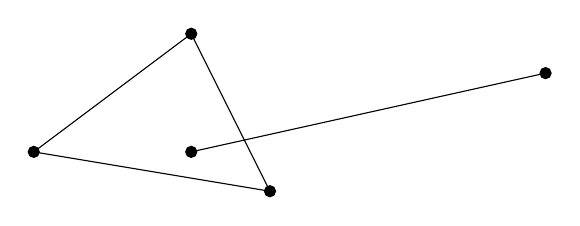
\begin{tikzpicture}

% Triangle component
\filldraw[black] (1,2) circle (2pt);  % Node A
\filldraw[black] (3,3.5) circle (2pt);  % Node B
\filldraw[black] (4,1.5) circle (2pt);  % Node C

\draw (1,2) -- (3,3.5);
\draw (3,3.5) -- (4,1.5);
\draw (4,1.5) -- (1,2);

% Two-node component
\filldraw[black] (3,2) circle (2pt);  % Node D
\filldraw[black] (7.5,3) circle (2pt);  % Node E

\draw (3,2) -- (7.5,3);

\end{tikzpicture}

}

\end{document}